\documentclass[12pt]{article}

\usepackage{graphicx}
\usepackage{paralist}
\usepackage{amsfonts}
\usepackage{amsmath}
\usepackage{hhline}
\usepackage{booktabs}
\usepackage{multirow}
\usepackage{multicol}

\newcommand{\be}{\begin{enumerate}}
\newcommand{\ee}{\end{enumerate}}

\oddsidemargin 0mm
\evensidemargin 0mm
\textwidth 160mm
\textheight 200mm
\renewcommand\baselinestretch{1.0}

\pagestyle {plain}
\pagenumbering{arabic}

\newcounter{stepnum}

%% Comments

\usepackage{color}

\newif\ifcomments\commentstrue

\ifcomments
\newcommand{\authornote}[3]{\textcolor{#1}{[#3 ---#2]}}
\newcommand{\todo}[1]{\textcolor{red}{[TODO: #1]}}
\else
\newcommand{\authornote}[3]{}
\newcommand{\todo}[1]{}
\fi

\newcommand{\wss}[1]{\authornote{blue}{SS}{#1}}

\title{Game Of Dots Specification}
\author{Anando Zaman}

\begin {document}

\maketitle
The purpose of this assignment is to design and specify modules for playing the game
Dots.  The modules listed in this document cover the Model, View, AND Controller portions of
the Model View Controller(MVC) design pattern.  The rules for Dots can be found
at the following web-page: https://www.gamesxl.com/think/two-dots\\

\noindent This Module Interface Specification (MIS) document contains modules, types, and methods for implementing the game known as Dots. The game incorporates a 6x6 grid with small colored nodes in each cell. The cells are characterized by any of the 4 colours (Red, Orange, Green, Blue) which are represented by the CellT module. The player is tasked with removing some fixed number of dots of a given colour with a certain number of moves. By default, the number of moves is 4 while the objectives are to get atleast 6 of a random color. The game ends after 4 or more moves has been exceeded, or when the player reaches the target objective. The GameBoard will be represented using the GameBoardT module that will use the CellT module. This will then be connected to the View module via Unit Tests to display the ASCII grid along with their score information to the user. As a added bonus, a controller module is also included in this specification which acts as an intermediate or communicator to update the model and view when the state information of the gameboard(model) changes.

\newpage

\section* {CellT Types Module}

\subsection*{Module}

CellT

\subsection* {Uses}

N/A

\subsection* {Syntax}

\subsubsection* {Exported Constants}

None

\subsubsection* {Exported Types}

CellT = \{R,O,G,B\}\\ 

\subsubsection* {Exported Access Programs}

\begin{tabular}{| l | l | l | l |}
\hline
\textbf{Routine name} & \textbf{In} & \textbf{Out} & \textbf{Exceptions}\\
\hline
getRandomCell & & CellT & \\
\hline
\end{tabular}

\subsection* {Semantics}

\subsubsection* {State Variables}

None

\subsubsection* {State Invariant}

None

\subsubsection* {Access Routine Semantics}

getRandomCell()):
\begin{itemize}
\item $out:= \thickspace CellT \thickspace of \thickspace any \thickspace of \thickspace the \thickspace avaiable \thickspace 4 \thickspace colors $
\end{itemize}

\subsubsection* {Assumptions \& Design Decisions}

\begin{itemize}
\item This class is essentially just used to create the various color types but it also contains the getRandomCell() method. This is a static method so that it can be accessed from any class without initlization of an object which allows the user to randomly select a cell color for later portions of the other modules(GameBoardT).

\end{itemize}

\newpage

\section* {GameBoardT ADT Module}

\subsection* {GameBoardT Template module}

GameBoardT()

\subsection* {Uses}

CellT

\subsection* {Syntax}


\subsubsection* {Exported Constants}

SIZE = 6 //Size of board in each direction

\subsubsection* {Exported Access Programs}

\begin{tabular}{| l | l | l | p{5cm} |}
\hline
\textbf{Routine name} & \textbf{In} & \textbf{Out} & \textbf{Exceptions}\\
\hline
new GameboardT &  & GameboardT & \\
\hline
move & $seq \thickspace of\thickspace seq(\mathbb{Z})$ & & IndexOutOfBounds\\ & & & IllegalArgument,\\ & & & NullPointerException\\
\hline
get\_moves & & $\mathbb{Z}$ &\\
\hline
get\_obj & & CellT, $\mathbb{Z}$ &\\
\hline
get\_score & & $\mathbb{Z}$ &\\
\hline
get\_boardT & & Seq of seq(CellT) &\\
\hline
game\_over & & $\mathbb{B}$ &\\
\hline
is\_win & & $\mathbb{B}$ &\\
\hline
\end{tabular}

\subsection* {Semantics}

\subsubsection* {State Variables}

$boardT$: seq [SIZE,SIZE] of CellT\\
$moves$: $\mathbb{N}$\\
$objectives$: seq of $CellT,\mathbb{N}$\\
$score$ : $\mathbb{N}$

\subsubsection* {State Invariant}

$objective[1] \leq 0$\\
$moves \leq 0$

\subsubsection* {Assumptions \& Design Decisions}

\begin{itemize}
\item The $GameBoardT$ constructor is called for each object instance before any other access routine is called for that object. The constructor can only be called once.

\item Right after the constructor, the $initialize\_board()$ method is called only once to initialize the grid, score, objectives, and moves. The default objective is to get 6 CellT.R with 4 single moves available to do this. The game cannot continue until this method is executed.

\item The local methods may be of use but it is up to the implementer to decide whether they are needed.

\item Additional public setters and getters methods are NOT needed for exported access programs as they are not required by the user to play or run the game. The only useful information to the user will be the existing getter methods that retrieve the game state information along with the move method which will allow them to connect the dots.

\item For better scalability, this module is specified as an Abstract Data Type (ADT) instead of an Abstract Object. This allows for multiple games to be created that can run independently from a different game while being tracked by the client concurrently.

\item It is assumed that to form a valid move, atleast 2 or more distinct adjacent cell coordinates have to be placed in the path array. This is because one cell on its own does not create a path as its destination is itself.

\item Each time the $initialize\_board$ is called, the default grid will be displayed (Refer to the Access Routine Semantics below for this grid/board). This was done versus randomly generating the colors for the cells because it ensures there are always some possible combinations that are valid. Having an initially randomized cellT generation can cause the off chance that there are no available paths to create on the grid. By having a predefined default grid, it makes it easier to test for correctness during Unit Tests. If the grid was instead randomly generated, the unit tests could prove to be difficult as the test cases would have to dynamically figure out valid paths to test.

\item Another assumption that was made is that there CANNOT be duplicate coordinates in the path arrays that are passed into the module. This means that every coordinate in the path arrays are unique and distinct. For example, [[1,2],[1,3],[2,3]] is valid but [[1,2],[1,2],[1,3],[2,3]] is not.

\item Another assumption is that the path arrays are given in order of adjacency of the cells to each other to simulate a path. For example; the user can input [[1,2],[1,3],[2,3],[2,4],[3,4]] which all lie on the same path and each are adjacent to its successor and predecessor cells. Lets take coordinate [1,3] from above as an example. This cell is adjacent to cell at [1,2] by being one unit to the right of it while also being adjacent to cell at coordinate [2,3] by being one unit above it. This is a valid path as it follows an adjacency cell format. An example of an invalid path could be [[1,2],[1,5],[4,5],[4,1],[1,3]]. This clearly doesn't form a valid path as the nodes are all over the place and are not adjacent to each other either.

\item The exceptions are only raised on the move method. This is because the move method is the mutator that is modifying the state variables such as the boardT variable. It was designed this way because the rest of the public methods here are getters which only return the value associated with the state variable. Getters would not return an error for these cases. Therefore, the exceptions are best suited for placement within the move method.

\item The exceptions also contain an error message. For example, NullPointerException has the following, $"please \thickspace enter \thickspace a \thickspace valid \thickspace path"$. This can be useful for the user to understand what went wrong. However, this additional component of the error message is completely optional and up to the implementer to decide.

\item It is also important to note that if an exception occurs, the boardT does not get modified or updated. So when executing the JUnit tests with expected exceptions, the board will be printed as if nothing changed.

\end{itemize}
\newpage

\subsubsection* {Access Routine Semantics}

GameboardT()):
\begin{itemize}
\item transition: $$ boardT := 
< \begin{array}{c}
< \mbox{CellT.R}, \mbox{CellT.R}, \mbox{CellT.R}, \mbox{CellT.B}, \mbox{CellT.R}, \mbox{CellT.R}>\\
< \mbox{CellT.O}, \mbox{CellT.R}, \mbox{CellT.R}, \mbox{CellT.R}, \mbox{CellT.B}, \mbox{CellT.O}>\\
< \mbox{CellT.B}, \mbox{CellT.B}, \mbox{CellT.O}, \mbox{CellT.G}, \mbox{CellT.G}, \mbox{CellT.G}>\\
< \mbox{CellT.G}, \mbox{CellT.R}, \mbox{CellT.R}, \mbox{CellT.G}, \mbox{CellT.O}, \mbox{CellT.B}>\\
< \mbox{CellT.B}, \mbox{CellT.B}, \mbox{CellT.R}, \mbox{CellT.O}, \mbox{CellT.G}, \mbox{CellT.B}>\\
< \mbox{CellT.B}, \mbox{CellT.B}, \mbox{CellT.R}, \mbox{CellT.O}, \mbox{CellT.G}, \mbox{CellT.B}>\\
\end{array} >
$$

$moves :=$ $4$\\
$objectives :=$ $CellT.Red, 6$\\
$score :=$ $0$\\

\end{itemize}

move(Seq of seq($\mathbb{Z}$)):
\begin{itemize}
\item transition:= $valid\_coordinate (path[0][0], path[0][1]) \thickspace \land \thickspace valid\_path(path[0][0],path[0][1],path)) \thickspace \land  \thickspace one\_direction(path) \thickspace \land \thickspace \lnot(game\_over()) \thickspace \land \thickspace \lnot(is\_win()) \thickspace \land \thickspace drop\_down\_cells(path) \thickspace \land \thickspace (dec\_moves()) \thickspace \land \thickspace update\_score(|path|) \thickspace \land \thickspace update\_obj(|path|) \thickspace \land \thickspace (get\_obj[0] = get\_boardT[path[0][0]][path[0][1]]$\\

\item exception: \\exc:= $((path = null) \thickspace \lor \thickspace (|path| = 0)) \rightarrow NullPointerException$\\ $| \thickspace\lnot (valid\_coordinate(path[0][0], path[0][1])) \rightarrow IndexOutOfBoundsException \thickspace$ \\ $| \thickspace \lnot(valid\_path(path[0][0], path[0][1],path) \thickspace = null) \thickspace \rightarrow \thickspace IndexOutOfBoundsException$\\ $| \thickspace \lnot(one\_direction(path)) \rightarrow IllegalArgumentException$ $\thickspace$
$| \thickspace game\_over() \thickspace \rightarrow
 \thickspace IllegalArgumentException$
\end{itemize}

\noindent get\_moves():
\begin{itemize}
\item output: $out := moves$
\item exception: None
\end{itemize}

\noindent get\_obj():
\begin{itemize}
\item output: $out := objectives$
\item exception: None
\end{itemize}

\noindent get\_score():
\begin{itemize}
\item output: $out := score$
\end{itemize}

\noindent get\_boardT():
\begin{itemize}
\item output: $out := boardT$
\end{itemize}

\noindent is\_win():
\begin{itemize}
\item output: $out := get\_obj()[1] \le 0$
\item exception: None
\end{itemize}

\noindent game\_over():
\begin{itemize}
\item output: $out := get\_moves() \le 0$
\item exception: None
\end{itemize}

\subsubsection* {Local Functions}
\textbf{set\_obj} : $\mathbb{Z}$ \\
set\_obj($i$) $\equiv$ $boardT.objective[1] := get\_obj()[1] - i$\\

\textbf{set\_score} : $\mathbb{Z}$ \\
set\_obj($i$) $\equiv$ $boardT.score := get\_score() + i$\\

\textbf{dec\_moves} : $\mathbb{Z}$ \\
set\_obj($i$) $\equiv$ $boardT.moves := get\_moves() - i$\\

\textbf{same-cell-data} : $\mathbb{Z}$ $\times$  $\mathbb{Z}$ $\times$ $\mathbb{Z}$ $\times$ $\mathbb{Z}$ $\rightarrow$ $\mathbb{B}$\\
same-cell-data$(start\_row, start\_col, row, col) \equiv get\_boardT()[start\_row][start\_col]$ 
= $get\_boardT()[row][col]$\\

\textbf{drop\_down\_cells($seq$)}: $Seq \thickspace of \thickspace Seq  \thickspace \mathbb{Z}$
\\drop\_down\_cells($seq$) $:= (seq : seq \thickspace of \thickspace (\mathbb{Z}) \thickspace | \thickspace i \in seq[0] \thickspace \land \thickspace j \in seq[1] : (boardT[i][j] := boardT[i-1][j]) \thickspace \land \thickspace (boardT[i-1][j] := CellT.random()))$\\

\textbf{valid\_coordinate}: $\mathbb{Z} \times \mathbb{Z} \rightarrow \mathbb{B}$ \\
valid\_coordinate(row,col) $\equiv$ $(row \ge 0) \thickspace \land \thickspace (row \le 6) \thickspace \land (col \ge 0) \thickspace \land \thickspace (col \le 6) $\\

\textbf{same-cell-data} : $\mathbb{Z}$ $\times$  $\mathbb{Z}$ $\times$ $\mathbb{Z}$ $\times$ $\mathbb{Z}$ $\rightarrow$ $\mathbb{B}$\\
same-cell-data$(start\_row, start\_col, row, col) \equiv boardT[start\_row][start\_col] = boardT[row][col]$\\\\\\

//Below method, checks if moving vertically or horizontally\\
//Returns false if moving Diagonally\\
\textbf{one\_direction}: seq of seq($\mathbb{Z}$)\\
one\_direction(path): $(i_1:\mathbb{N},i_2:\mathbb{N} \thickspace | \thickspace i_1 \in [1,2,...|path|-1] \thickspace \land \thickspace (i_2:=i_1-1) \thickspace \land \thickspace ((path[i_1][0] = path[i_2][0]) \thickspace \lor \thickspace (path[i_1][1] = path[i_2][1]) \thickspace : \thickspace true)$\\

\textbf{valid\_path}: $\mathbb{Z} \thickspace \times \mathbb{Z} \thickspace \times \thickspace seq \thickspace of \thickspace seq(\mathbb{Z})$ \\
valid\_path(start\_row, start\_col, path): $\equiv$ $(i : \mathbb{N} \thickspace | \thickspace i \thickspace \in \thickspace [0,1,2,...|path|-1] \thickspace \land \thickspace$\\ $valid\_coordinates(path[i][0],\thickspace path[i][1]) \thickspace \land \thickspace same\_cell\_data(path[0][0],\thickspace path[0][1],\thickspace path[i][0],\thickspace path[i][1]))$\\
Otherwise returns the coordinate that it failed at. ie; $(path[i][0],path[i][1])$\\




\newpage

\section* {View Module}

\subsection*{View Module}

View Module

\subsection* {Uses}

\noindent GameboardT
\subsection* {Syntax}

\subsubsection* {Exported Access Programs}

\begin{tabular}{| l | l | l | l |}
\hline
\textbf{Routine name} & \textbf{In} & \textbf{Out} & \textbf{Exceptions}\\
\hline
print\_boardT & Seq of seq($CellT$) & print grid row by row &\\
\hline
print\_info & CellT, $\mathbb{Z}$, $\mathbb{Z}$, $\mathbb{Z}$ & printf(objective, score, moves) & \\
\hline
\end{tabular}

\subsubsection* {Access Routine Semantics}

print\_boardT()):
\begin{itemize}
\item $out:= \thickspace Prints\thickspace the \thickspace grid \thickspace to \thickspace the \thickspace console \thickspace row \thickspace by \thickspace row. $
\end{itemize}

print\_info()):
\begin{itemize}
\item $out:= \thickspace Prints \thickspace the \thickspace state \thickspace variables \thickspace objective \thickspace CellT, \thickspace objective \thickspace target, \thickspace score, \thickspace moves $
\end{itemize}

\subsection* {Assumption and Explanation}
\begin{itemize}
\item This module will be used to output the grid/board while the user is playing. 
\item This class has two public methods. A View object must be created in order to output information to the user via the console. 
\item The $print\_boardT()$ method will just print the $6x6$ grid to the screen each time a move is executed. The $print\_info$ method takes $objective\_cell, \thickspace objective\_target, \thickspace score, \thickspace$\\ $ and \thickspace moves$. This will let the user be aware of how many moves they have remaining along with their objectives and score information. 
\end{itemize}


\newpage

\section* {Controller Module}

\subsection*{Controller Module}

Controller Module

\subsection* {Uses}

\noindent GameboardT, View
\subsection* {Syntax}

\subsubsection* {Exported Access Programs}

\begin{tabular}{| l | l | l | p{5cm} |}
\hline
\textbf{Routine name} & \textbf{In} & \textbf{Out} & \textbf{Exceptions}\\
\hline
new Controller & GameBoardT, View & Controller & \\
\hline
execute\_move & $seq \thickspace of\thickspace seq(\mathbb{Z})$ & & IndexOutOfBounds\\ & & & IllegalArgument,\\ & & & NullPointerException\\
\hline
get\_game\_moves & & $\mathbb{Z}$ &\\
\hline
get\_game\_obj & & CellT, $\mathbb{Z}$ &\\
\hline
get\_game\_score & & $\mathbb{Z}$ &\\
\hline
get\_game\_boardT & & Seq of seq(CellT) &\\
\hline
game\_over & & $\mathbb{B}$ &\\
\hline
is\_win & & $\mathbb{B}$ &\\
\hline
\end{tabular}

\subsection* {Semantics}

\subsubsection* {State Variables}

$gameboard$: $new \thickspace GameboardT$\\
$View$: $new \thickspace View$\\

\subsubsection* {Access Routine Semantics}

Controller($gameboard$, $view$):
\begin{itemize}
\item transition: \\$gameboard := gameboard$\\
				  $view := view$\\

\end{itemize}

execute\_move(path)):
\begin{itemize}
\item transition:= $gameboard.move(path) $\\

\item exception: These exceptions propagate from GameBoardT module. Look at that module for more details\\exc:= $((path = null) \thickspace \lor \thickspace (|path| = 0)) \rightarrow NullPointerException$\\ $| \thickspace\lnot valid\_coordinate(path[0][0], path[0][1]) \rightarrow IndexOutOfBoundsException \thickspace$ \\ $| \thickspace \lnot(valid\_path(path[0][0], path[0][1],path) \thickspace = null) \thickspace \rightarrow \thickspace IndexOutOfBoundsException$\\ $| \thickspace !one\_direction(path) \rightarrow IllegalArgumentException$ $\thickspace$
$| \thickspace game\_over() \thickspace \rightarrow
 \thickspace IllegalArgumentException$
\end{itemize}

\noindent get\_game\_moves():
\begin{itemize}
\item output: $out := gameboard.get\_moves()$
\item exception: None
\end{itemize}

\noindent get\_game\_obj():
\begin{itemize}
\item output: $out := gameboard.get\_obj()$
\item exception: None
\end{itemize}

\noindent get\_game\_score():
\begin{itemize}
\item output: $out := gameboard.get\_score()$
\end{itemize}

\noindent get\_game\_boardT():
\begin{itemize}
\item output: $out := gameboard.get\_boardT()$
\end{itemize}

\noindent is\_win():
\begin{itemize}
\item output: $out := get\_game\_obj()[1] \le 0$
\item exception: None
\end{itemize}

\noindent game\_over():
\begin{itemize}
\item output: $out := get\_game\_moves() \le 0$
\item exception: None
\end{itemize}

\subsection* {Assumption and Explanation}
\begin{itemize}
\item This module will always run $Controller$ method before every other method. It will only be run once.

\item The exceptions of the controller are that of the GameBoardT module as it propagates through when the Controller uses it.

\end{itemize}

\newpage

\section* {Design Overview and Critique}

After completing the design specification, there are a few topics to discuss in terms of software quality. The specification was designed with the properties of good module interface design which are consistency, essentiality,
generality, minimality, high cohesion and low coupling. \\

The specification is consistent due to the same naming conventions along with general ordering of parameters in arguments. The naming conventions for functions and state variables in GameBoardT are descriptive and follow the general rules for naming conventions in java. Thus, it is consistent. This is true for all the other modules as well.\\

In terms of essentiality, all the modules are essential as they do not have functions executing redundant features. The controller for the most part just uses the functions supplied from the GameboardT and View objects passed as a parameters. This might seem redundant as there are similar methods in the Controller that are also found in the GameboardT module. However, it is alright in this case because the controller must do this as it is extracting data from model to update the view.\\

In terms of generality, the spec is not very general as no generics and comparables were implemented. The game is only being played with 6X6 grid specifically filled with CellT data. Since the Dots game is specifically played using Cell colors versus numbers or other data in the cells, it is alright for the specification to not be general in this case.\\

In addition to this, although minimality is conserved for majority of the specification, it is not for some portions. This is for good reason. The GameboardT module violates minimality so that multiple state variables can be updated at once without needing to call seperate setter methods manually each time a move is run. This makes the game easier to play and work with as the setter methods do not have to be called each time manually. For this reason, it was chosen to violate minimality in the GameBoardT module of the specification.\\

 It is often good practice to have high cohesion and low coupling in modular design. High cohesion is enforced as the modules are closely related to each other in various aspects. However, coupling is relatively high as the view strongly depends on the model to get data to output to the user. The view does not have a default game board to display on its own as all that data is collected and set by the GameboardT. The purpose of the view is so that it can update the user with the state changes of the game board. Thus, the view has to be closely related and strongly dependent on the changes of the model\\
 
Finally, in terms of information hiding, the specification satisfied this quality. Information hiding and abstraction is important so that only the relevant information and methods are available to the client. The client does not care about how the the modules are implemented, they only care about using it. For this reason, only the most necessary access routines were selected to be exported and publicly available for the user to use. Specifically for the GameBoardT module, this consisted of a few getter methods for the states of the gameboard, $win$ and $game\_over$, and the $move()$ methods. The rest of the information of the modules were kept private and any additional helper methods were also kept private. This way, the client can play the game without needing to worry the specific details of how the modules work.\\
 
 Although the software qualities above are great to follow, they do not always have to be followed. Depending on the specific situation and use cases, certain qualities can be violated. This concludes the design critique portion.

\newpage

\section* {Design Questions}
\be  

  \item Please compare and contrast the proxy, strategy and adapter design patterns. The
UML diagrams for each look similar, but the purpose of the patterns are different.
2
What do the patterns have in common? How are they different? In which situations
would you use each pattern?

\textbf{Solution:} \\ There are a few key differences and similarities between the proxy, strategy, and adapter patterns. For one, Proxy and Adapter are part of the structural classification of design patterns which are concerned with how class and objects are composed, to form larger structures. On the other hand, the strategy pattern is part of the behavioural classification which has more to do with describing how objects interact with each other typically at runtime.\\

The Proxy design pattern is kind of like the middle man or intermediary to communicate with the client while the adapter is more concerned towards making incompatible classes work together by converting the interfaces. They are both similar in that they provide the ability to build larger complex structures from smaller ones. \\

You would typically use the proxy pattern when direct access to a object is not ideal due to factors such as security. Using a proxy can get around this problem by creating an intermediary class. A good example is when you get your bi-weekly paycheck. Sure, your employer could give you your paycheck in direct cash but that could be dangerous. If others find out, you would likely be approached by others trying to steal your money. It could result in severe injuries or worse, death. A paycheck can be a proxy in the banking software system which can ensure that only you get that money as it is issued to your name and back account.\\

As explained earlier, the adapter pattern is used when you are dealing with incompatible classes that are trying to work together. The adapter essentially wraps an existing class with a new interface to ensure compatibility. A good application could be trying to reuse old incompatible classes in a program to build a larger complex system. The adapter can fix the compatibility issues, allowing the software development to progress.\\

The Strategy pattern deals with encapsulating each algorithm from a family of algorithms, and makes them interchangeable for use at run-time. This can be useful if you are unsure the specific algorithm to use for different cases. For example, assume you are given a small unordered array to sort with few inversions. Since the dataset is small with only few inversions, it may be useful to use something like \emph{InsertionSort} or \emph{SelectionSort} since they use less memory versus something like \emph{QuickSort} or \emph{MergeSort}. However, if you were instead tasked with sorting a large unordered array, \emph{InsertionSort} or \emph{SelectionSort} may not be ideal as they take long computation times due to $O(N)$ time complexity. It maybe beneficial to use \emph{QuickSort} since it has $O(N log N)$ time complexity even if it takes $O(log(N))$ extra space as it is much faster in computation. Situations like this where the scenarios are not always the same, may benefit from using the strategy design pattern to pick the most optimal algorithm at run time.\\

\item    CODE shown below\\
\begin{center}
	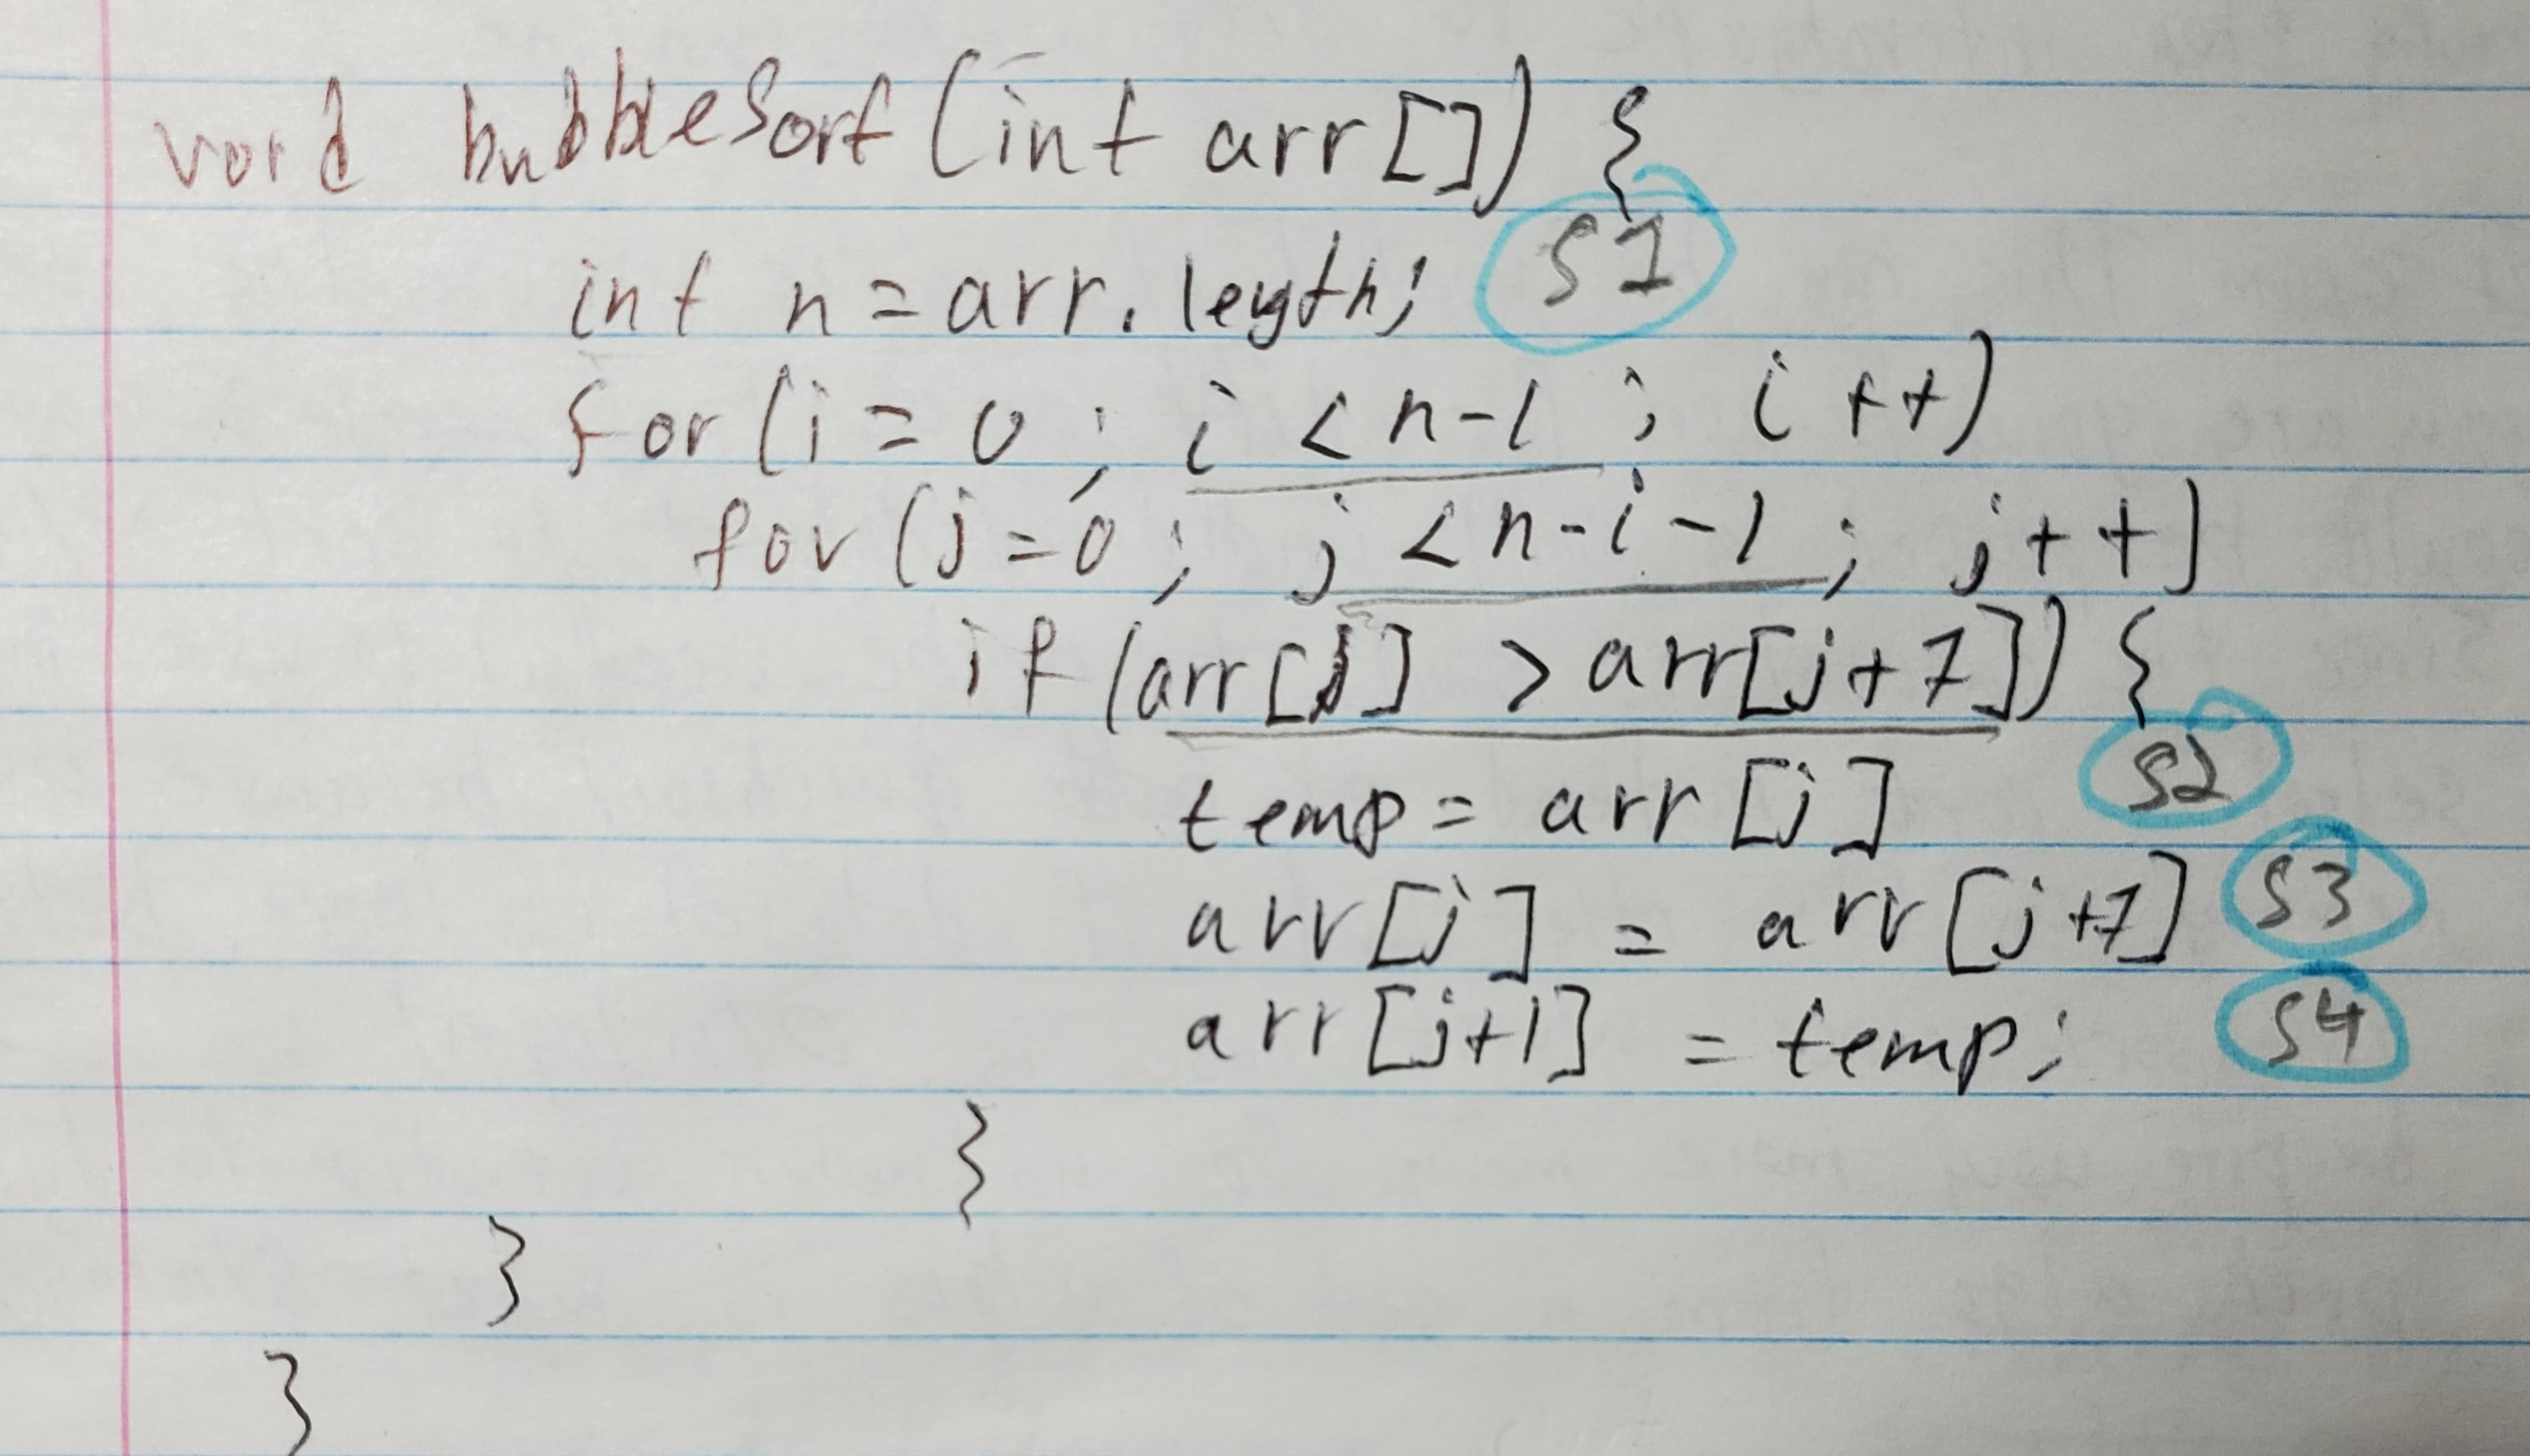
\includegraphics[scale = 0.1]{code.jpg}
	\end{center}
Flow Chart Shown below:\\
\begin{center}
	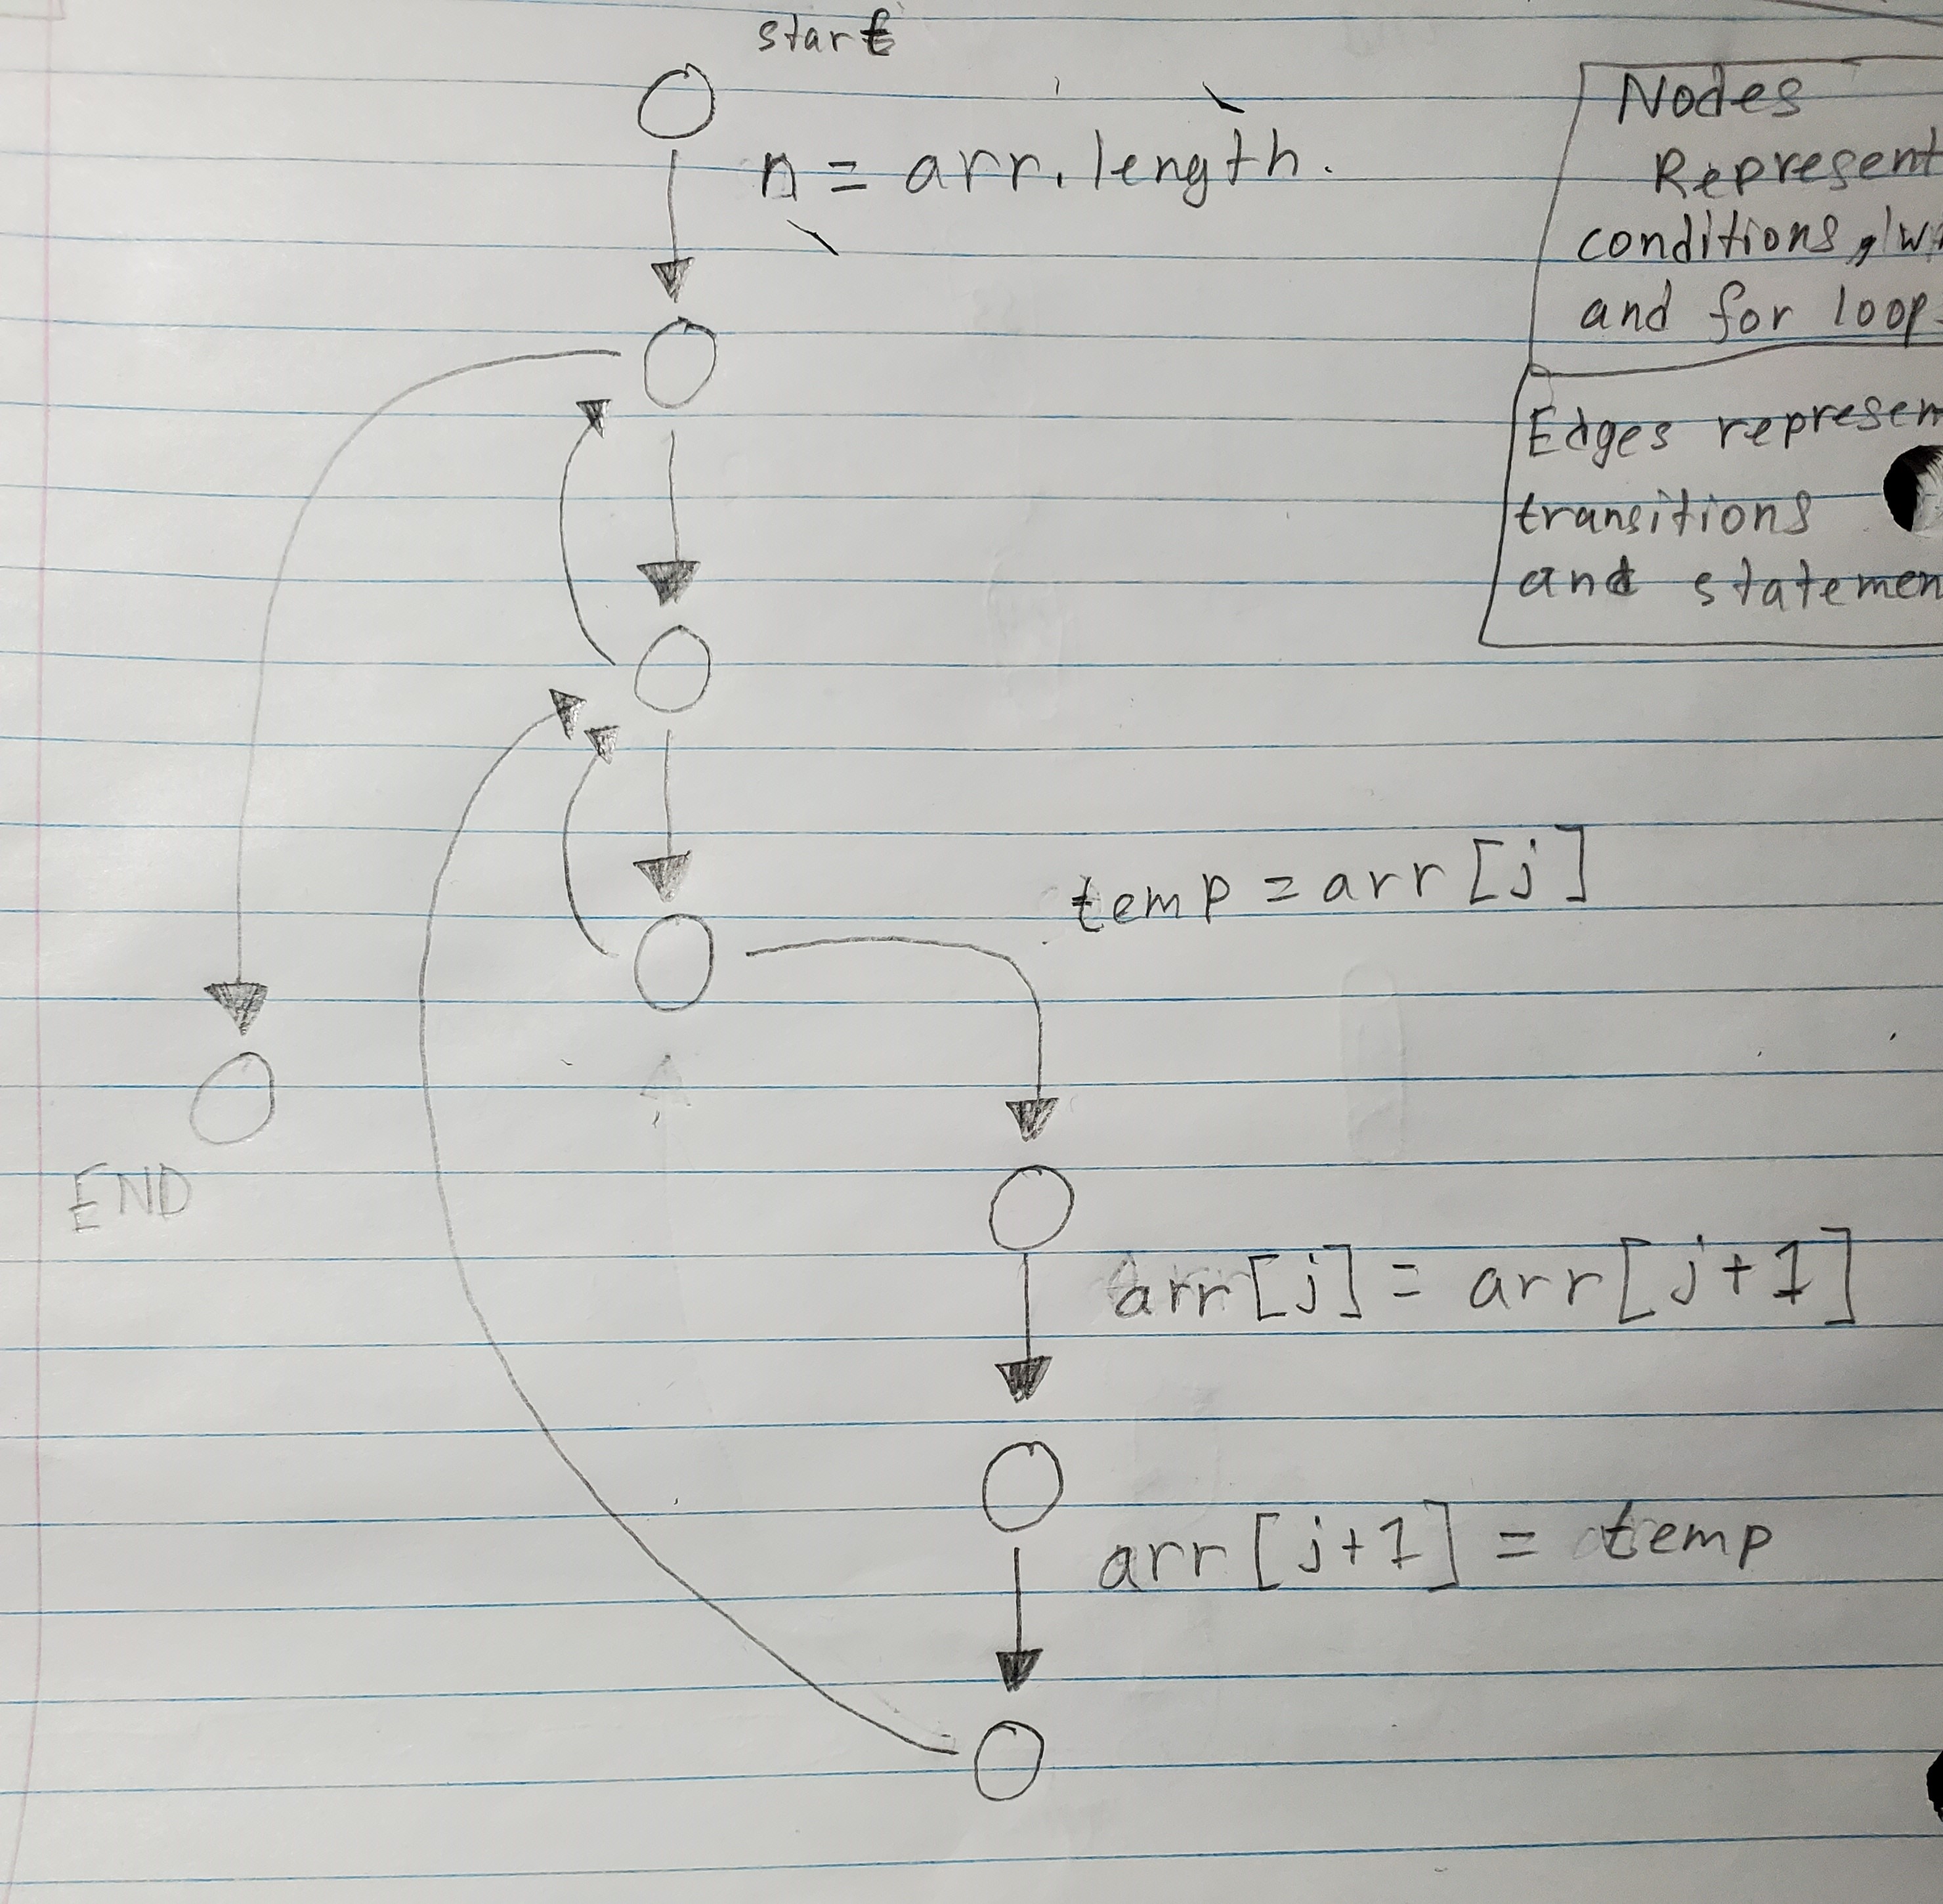
\includegraphics[scale = 0.12]{flowdiagram.jpg}
	\end{center}

\ee


\end{document}